\subsection{Package della componente Controller}
	\begin{center}
		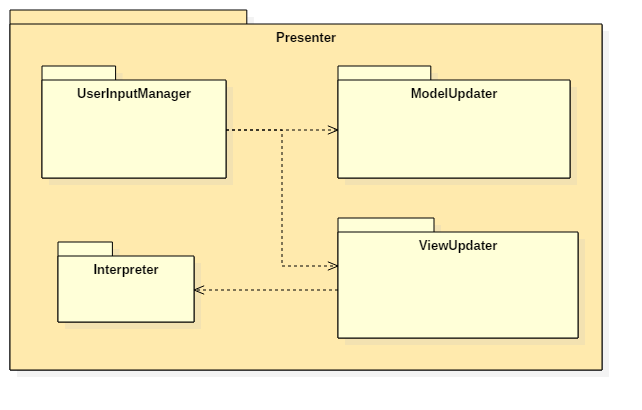
\includegraphics[scale=0.6]{../images/PresenterPackage.png}
	\end{center}
	Gli elementi del package collaborano e interagiscono con l'obiettivo comune di trattare il flusso di dati tra View e Model e mantenere aggiornato lo stato di entrambi. \\
	Il package del Presenter contiene i seguenti sub-packages:
	\begin{itemize}
	\item \textbf{UserInputManager}:
	Il package \emph{UserInputManager} gestisce gli input degli utenti ricevuti dalla View, realizzando la logica dell'applicazione web. Per svolgere il proprio compito si interfaccia con il package \emph{Updaters} per aggiornare e interagire con View e Model. \\
	Il package contiene al suo interno le classi:
	\begin{itemize}
		\item \textit{InputManager}
		\item \textit{Input}
		\item\textit{CreateQuiz}
		\item\textit{AddQuestion}
		\item\textit{RemoveQuestion}
		\item\textit{SaveQuiz}
		\item\textit{CreateQuestion}
		\item\textit{SaveQuestion}
		\item\textit{DeleteQuestion}
		\item\textit{ChooseQuiz}
		\item\textit{StartQuiz}
		\item\textit{NextQuestion}
		\item\textit{PreviousQuestion}
		\item\textit{EndQuiz}
		\item\textit{ViewProfile}
		\item\textit{UpdateProfile}
		\item\textit{ViewQMLTutorial}
		\item\textit{ViewQuizList}
	\end{itemize}	
	\item \textbf{Updaters}:
	Il package \emph{Updaters} ha la responsabilità di aggiornare View e Model in risposta agli input utente. per svolgere i suoi compiti collabora con i packages \emph{QuizManger} e \emph{QuestionManager}. Il package contiene al suo interno le classi:
	\begin{itemize}
		\item \textit{Updater}
		\item \textit{ModelUpdater}
		\item \textit{ViewUpdater}
	\end{itemize}
	
	\item \textbf{QuestionManager}:
	Il package \emph{QuestionManager} espone le funzionalità necessarie alla creazione e gestione di domande. Per permettere al package di essere estendibile in futuro con domande in diversi formati, le classi al suo interno sono organizzate seguendo il pattern \emph{Abstract Factory}. \\
	Il package contiene al suo interno le classi:
	\begin{itemize}
		\item \textit{QuestionFactory}
		\item \textit{Question}
		\item \textit{QML2HTMLFactory}
		\item \textit{HTMLQuestion}
		\item \textit{Translator}
	\end{itemize}
	
	\item\textbf{QuizManager}:
	Il Package \emph{QuizManager} espone le funzionalità necessarie alla creazione e gestione di quiz, collaborando con il package \emph{QuestionManager}. Per disaccoppiare la creazione di un quiz dalle domande che lo compongono, la classi all'interno del package seguono la struttura del design pattern \emph{Builder}.\\ 
	Il package contiene al suo interno le classi:
	\begin{itemize}
		\item \textit{QuizDirector}
		\item \textit{QuizBuilder}
		\item \textit{Quiz}
	\end{itemize}
	
	\item \textbf{Interpreter}:
	Il package \emph{Interpreter} è responsabile della traduzione di testo QML in codice HTML5 visualizzabile da browser. Per permettere al package di essere estendibile in futuro con nuovi tipi di "Interpreter", le classi al suo interno sono organizzate seguendo il pattern \emph{Abstract Factory} . \\
	Il package contiene al suo interno le seguenti classi:
	\begin{itemize}
	\item \textit{Interpreter}
	\item \textit{InterpreterFactory}
	\item \textit{QMLInterpreterFactory}
	\item \textit{QMLInterpreter}
	\item \textit{QML2HTMLInterpreter}
	\end{itemize}
	
	\end{itemize}